\documentclass[11pt]{article}
%\setlength{\oddsidemargin}{0in}
%\setlength{\topmargin}{0.0in}
%\setlength{\textwidth}{6.7in}
%\setlength{\textheight}{8.5in}
%\usepackage{graphicx}
\usepackage{enumitem}
\usepackage{mathtools}
\usepackage[usenames,dvipsnames]{xcolor}

\usepackage{geometry}
 \geometry{
 letterpaper,
 textwidth=6.8in
 }
\usepackage[utf8]{inputenc}
%\usepackage{libertine}
%\usepackage{libertinust1math}
\usepackage[libertine,cmintegrals,cmbraces,vvarbb]{newtxmath}
%\usepackage{newtxmath}
%\usepackage[osf]{ebgaramond}
\usepackage[T1]{fontenc}
%\usepackage{palatino}
\usepackage{microtype}

\usepackage{fancyhdr}
\usepackage[colorlinks=true]{hyperref}

\newcommand{\ep}{e^{-i\phi}}

\pagestyle{fancy}
\fancyhf{}
\fancyhead[RE,LO]{\textcolor{BlueViolet}{Gravitational Waves}}
\fancyhead[LE,RO]{ph237: 2018}

\fancyfoot[RE,LO]{\textcolor{Orange}{Caltech}}
\fancyfoot[LE,RO]{\textcolor{Orange}{Physics, Math, and Astronomy}}

%\input mydefs.tex
\def\vev#1{\left\langle #1\right\rangle}
\def\hb{\hfill\break}

\begin{document}
%



\medskip

\begin{enumerate}

\item
{\bf Fabry-Perot Cavity} \\
There exists a Fabry-Perot cavity with a length of 4000\,m. The \emph{power} transmission, $T_I$, of the input mirror is 1\% and the transmission of the end mirror, $T_E$, is 10\,ppm. The cavity is illuminated from the input side with a 100\,W laser having a wavelength of 437\,nm.
\begin{itemize}

\item[\bf a)] {\bf Using the steady state fields approach, solve for the transmitted \emph{power} as a function of cavity length.}

\begin{figure}[t]
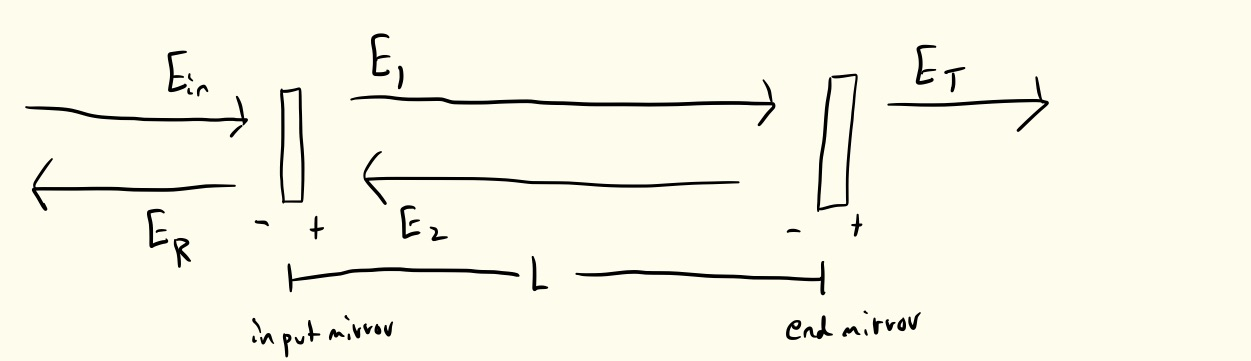
\includegraphics[width =1\columnwidth]{FPdiag}
\caption{
}
\label{fig:FP}
\end{figure}

The Fabry-Perot Cavity is schematically drawn in figure \ref{fig:FP}

To use the steady state fields approach, we make the ansatz that the field is a superposition of a left-going wave and a right going wave to the left of the cavity (with amplitudes $E_{\rm in}$ and $E_{\rm R}$ in the figure), a superposition of a left-going wave and a right going wave inside the cavity  (with amplitudes $E_{1}$ and $E_{2}$ in the figure) and a right-going wave to the right of the cavity ( (with amplitude $E_{\rm T}$).

To use the steady state field approach we have to make sure the ansatz is consistent with the reflectivity and transmissivity at each mirror. This means we solve the system of equations (for $E_1$, $E_2$, $E_{\rm R}$ and $E_{\rm T}$ as a function of L , $\omega$, and $E_{\rm In}$)
\begin{align}
E_{\rm R}&=-r_I E_{\rm In} \\
E_1&=t_I E_{\rm In}+r_I E_2 \\
E_2& =-r_E e^{-2i\phi}E_1 \\
E_{\rm T}&=t_E e^{-i\phi}E_1,
\end{align}
where the phase $\phi =\omega_0L/c$ and the lower case $t$ and $r$ are the amplitude transmissivity and reflectivity (which are the square roots of the energy transmissivity and reflectivity). 
This solution for the transmitted field is 
\begin{align}
E_{\rm T}=\frac{t_Et_I e^{-i\phi}}{1+r_Ir_E e^{-2i\phi}}E_{\rm In}
\end{align}

The power is proportional to the field modulus squared $P\propto |E|^2$; Hence the transmitted power is
\begin{align}
P_T&=\left |\frac{t_Et_I e^{-i\phi}}{1+r_Ir_E e^{-2i\phi}} \right |^2P_{\rm In} \nonumber \\
&=\frac{T_ET_I}{1+R_IR_E+2r_Ir_E\cos(2\phi)}
,
\end{align}
where $P_{\rm In}$ is the laser power,

\item[\bf b)] {\bf Draw a diagram of the cavity, label each of the nodes, and write down the Adjacency Matrix, $A$, for the Fabry-Perot cavity. Solve for the System Matrix, $G$ using Mathematica or Python or otherwise, and show how one of the elements of $G$ can be used to find the solution in part a).}

\begin{figure}[t]
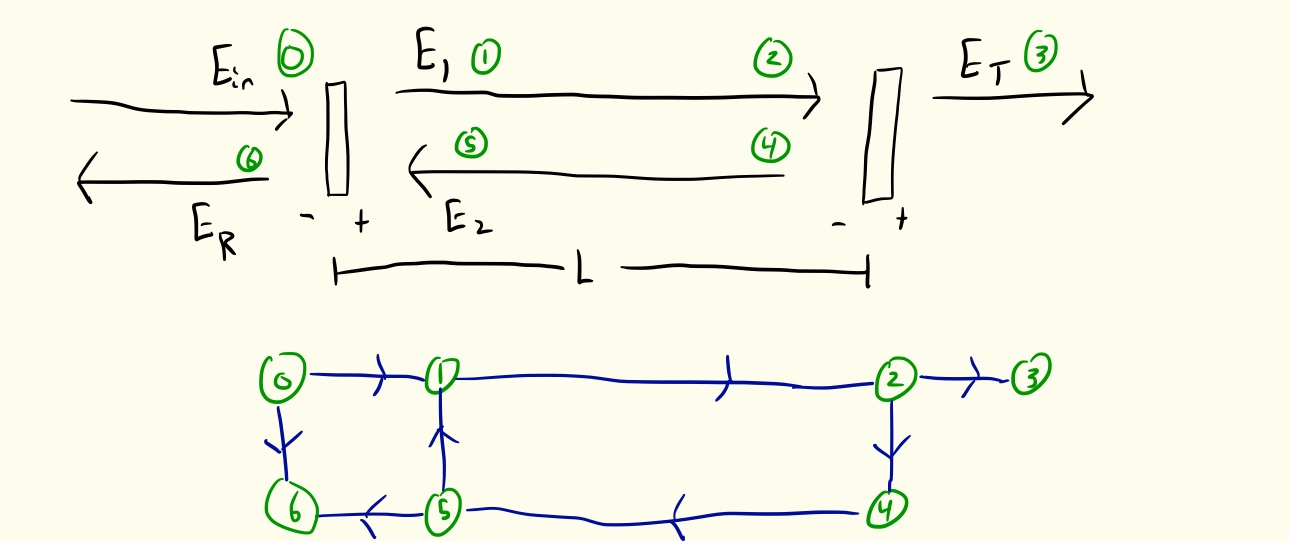
\includegraphics[width =1\columnwidth]{FPgraph}
\caption{
}
\label{fig:FPgraph}
\end{figure}

The translation of the optical system into a directed graph is shown in figure \ref{fig:FPgraph}

Recall that the adjacency matrix is defined by
\begin{align}
A_{ij}=\text{value of connection connecting node j to node i}
\end{align}

For the Fabry Perot Cavity in figure \ref{fig:FPgraph}, the nonzero components of the adjacency matrix are
\begin{align}
&A_{10}=t_I ,& &A_{15}=r_I,& & A_{21}=e^{-i\phi},& &A_{32}=t_E,& \nonumber \\
&A_{42}=-r_E,&
&A_{54}=e^{-i\phi},&
&A_{60}=-r_I,&
&A_{65}=t_I&
\end{align}

The vector of fields $\vec E =(E_0, \dots, E_6)^T$ obeys
\begin{align}
\vec E =A \vec E +\vec E_{\rm Inj},
\end{align}
where  the vector of injected fields is (in this case) $\vec E_{\rm Inj}=(E_{\rm In},\dots)^T$. This means that we can use the system matrix $G=(1-A)^{-1}$ to find the field at any of the node locations via
\begin{align}
\vec E =G \vec E_{\rm Inj} .
\end{align}
Performing the matrix multiplication, we see that
\begin{align}
E_i=G_{i0}E_{\rm In}.
\end{align}

An attached mathematica notebook computes the system matrix (symbolically).

\end{itemize}

\item
{\bf Frequency Response} \\
In this problem we will compute the frequency response of a LIGO-like interferometer to gravitational waves. Assume that the results from above still hold.
\begin{itemize}

\item[\bf a)] {\bf Assume that we now drive the end mirror with a sinusoidal modulation having an amplitude of $x_0$ and a frequency, $\omega$. Write down an expression for the fields reflected from the mirror, utilizing the Jacobi-Anger expansion.}

\begin{figure}[t]
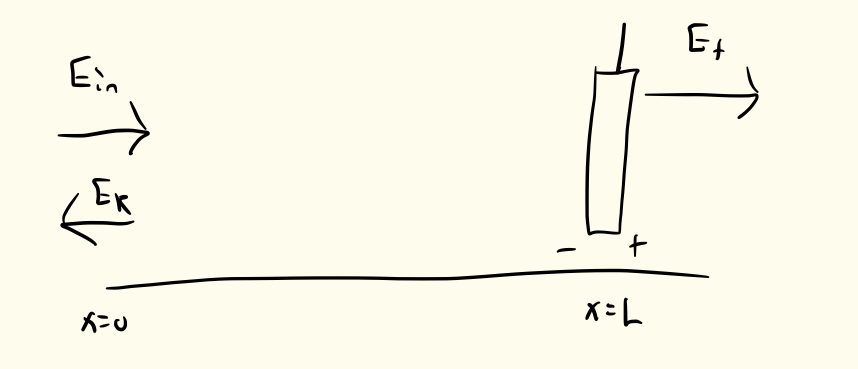
\includegraphics[width =1\columnwidth]{Driven}
\caption{
}
\label{fig:Driven}
\end{figure}

As is shown in fig \ref{fig:Driven}, suppose the central location of the mirror is $x=L$ and it is driven so that is position becomes $x=L+\delta L$, with $\delta L =x_0 \cos \omega t$. We calculate the values of the reflected field $E_{\rm R}$ (referred to at $x=0$) in terms of the ingoing field $E_{\rm In}$ (also referred to at $x=0$).

At the mirror location $x=L+\delta L$ the reflected field is simply $-r$ times the ingoing field evaluated at the mirror. The propagation to the mirror from $x=0$ contributes a phase factor $e^{-i\phi}$ and the propagation from the mirror to $x=0$, also contributes a phase factor of $e^{-i\phi}$, where $\phi=\omega_0(L+\delta L)/c=\omega_0(L+x_0\cos\omega t)/c$ and $\omega_0$ is the light frequency. Hence the reflected field is
\begin{align}
E_R&=-r_E e^{-2i\phi}E_{\rm In} 
=-r_E e^{-2i\omega_0L/c}e^{-2i x_0 \cos (\omega t)/c} E_{\rm In}
\end{align}
Taylor expanding in small $x_0$ (at fancy restaurants they call this utilizing the Jacobi-Anger expansion)
\begin{align}
E_R=-r_E e^{-2i\omega_0 L/c}\left[1-i\frac{x_0\omega_0}{c}(e^{i\omega t}+e^{-i\omega t})\right]E_{\rm In} \label{eq:side}
\end{align}

Note if we restore the time dependent factor $e^{i\omega_0t}$ that the first term has a time dependence $e^{i\omega_0t}$ (and is simply the reflected field when there is no modulation) while the second two terms are sideband fields with the time dependence $e^{i(\omega_0\pm\omega)t}$.

\item[\bf b)] {\bf Use your knowledge of the \emph{frequency dependent} System Matrix derived above to compute an expression for the transmitted power. Make a plot of the \emph{transfer function} of the transmitted power as a function of modulation frequency (the y-axis should be in units of Watts/meter).
\textbf{Hint:} Remember that the transmitted field will be the sum of the DC fields (computed above) and the AC fields}.

Now consider the Fabry Perot Cavity of problem one and imagine that we modulate the end mirror with $\delta L =x_0 \cos\omega t$. From part (a), we know that this produces sideband fields at node 4, i.e
\begin{align}
E_4=-r_E E_2+ir_E\frac{x_0\omega_0}{c}(e^{i\omega t}+e^{-i\omega t})E_{2},
\end{align}
where because of the optical set-up, we have set $L=0$ in Eq.~\eqref{eq:side}. As we are working to first order in the amplitude modulation, we can take $x_0=0$ when we evaluate $E_2$ the second term. From problem 1, when $x_0=0$, we know how to evaluate $E_2$ in terms of $E_{\rm In}$ and the system matrix $E_2=G_{20}(\omega_0)E_{\rm in}$. Hence
\begin{align}
E_4=-r_E E_2+ir_E\frac{x_0\omega_0}{c}(e^{i\omega t}+e^{-i\omega t})G_{20}(\omega_0)E_{\rm in}.
\end{align}
Here we are now writing the system matrix $G(\omega)$ as a function of frequency, with the frequency dependence coming from the frequency dependent phase $\phi(\omega)=\omega L/c$. Thus we see that we are effectively injecting fields at the sideband frequencies $\omega_0\pm \omega$ at node 4. The system matrix evaluated at the sideband frequencies also governs how light at the sideband frequencies propagates through the optical system. Thus we can write the complete field (with it's time dependence) as 
\begin{align}
\vec E(t)&=G(\omega_0)
\begin{bmatrix}
E_{\rm In} \\ 0 \\0 \\0 \\0 \\0 \\0
\end{bmatrix}
e^{i\omega_0 t} \nonumber \\
&+G(\omega_0 +\omega)
\begin{bmatrix}
0 \\ 0 \\ 0 \\0 \\ ir_EG_{20}(\omega_0)E_{\rm In}x_0\omega_0/c \\ 0 \\0
\end{bmatrix}
e^{i(\omega_0+\omega)t}
+G(\omega_0 -\omega)
\begin{bmatrix}
0 \\ 0 \\ 0 \\0 \\ ir_EG_{20}(\omega_0)E_{\rm In}x_0\omega_0/c \\ 0 \\0
\end{bmatrix}
e^{i(\omega_0-\omega)t}
\end{align}

Performing the matrix multiplication yields a transmitted field (including all of the time dependence) of
\begin{align}
E_T(t)&=G_{30}(\omega_0)E_{\rm In}e^{i\omega_0 t} \nonumber \\
&+G_{34}(\omega_0+\omega)ir_EG_{20}(\omega_0)x_0\frac{\omega_0}{c}E_{\rm In}e^{i(\omega+\omega_0)t}
+G_{34}(\omega_0-\omega)ir_EG_{20}(\omega_0)x_0\frac{\omega_0}{c}E_{\rm In}e^{i(-\omega+\omega_0)t} \label{eq:ETmod}
\end{align}

Thus we see that the transmitted field also has components at the carrier frequency $\omega_0$ and and the sideband frequencies $\omega_0\pm \omega$.

This produces an output power with a DC component  (computed in problem 1) and a slowly varying (relative to the carrier frequency) modulation at $\omega$. Namely, anytime the complex electric field is of the form
\begin{align}
E(t)=E_0e^{i\omega_0 t}+E_+e^{i(\omega_0+\omega)t}+E_-e^{i(\omega_0-\omega)t},
\end{align}
with $E_\pm\ll E_0$, then
the power is
\begin{align}
P&\propto |E|^2 \nonumber \\
&=|E_0|^2+E_0 e^{i\omega_0 t}(E_+^*e^{-i(\omega_0+\omega)t}+E_-^*e^{i(\omega_0+\omega)t}) +E_0^* e^{-i\omega_0 t}(E_+e^{i(\omega_0+\omega)t}+E_-e^{-i(\omega_0+\omega)t}) +\mathcal{O}(E_\pm^2) \nonumber \\
&=|E_0|^2+e^{i\omega t}\left[E_0^*E_++E_0E_-^*\right]+e^{-i\omega t}\left[E_0E_+^*+E_0^*E_-\right] \nonumber \\
&=|E_0|^2 +2A\cos(\omega t+\delta),
\end{align}
where $A$ and $\delta$ are the amplitude and phase of $E_0^*E_++E_0E_-^*=Ae^{i\delta}$.

The field in Eq.~\eqref{eq:ETmod} is off this form with 
\begin{align}
&E_0=G_{30}(\omega_0)E_{\rm In},& &E_{\pm}=ir_Ex_0\frac{\omega_0}{c}G_{34}(\omega_0\pm \omega)G_{20}(\omega_0)E_{\rm In}&
\end{align}
Note both $E_0$ and $E_{\pm}$ are proportional to $E_{\rm in}$. Note that both $A$ and $|E_0|^2$ are proportional to $|E_{\rm In}|^2$ or equivalently the input power $P_{\rm In}$. Hence, we can write
\begin{align}
P_T=|G_{30}(\omega_0)|^2P_{\rm In}+\Delta P\cos(\omega t+\phi),
\end{align}
where 
\begin{align}
\Delta P e^{i\phi}&=2G^*_{30}(\omega_0)ir_Ex_0\frac{\omega_0}{c}G_{34}(\omega_0+\omega)G_{20}(\omega_0)+2G_{30}(\omega_0)(ir_Ex_0\frac{\omega_0}{c}G_{34}(\omega_0-\omega)G_{20}(\omega_0))^*P_{\rm In} \nonumber \\
&=2ir_Ex_0\frac{\omega_0}{c}\left[G^*_{30}(\omega_0)G_{34}(\omega_0+\omega)G_{20}(\omega_0)-G_{30}(\omega_0)G^*_{34}(\omega_0-\omega)G^*_{20}(\omega_0)\right]P_{\rm in},
\end{align}
We consider the transfer function from modulation amplitude to power to be $\Delta P/x_0$. An attached python code computes $\Delta P/x_0$. Figure \ref{fig:2b} shows  $\Delta P/x_0$ as a function of modulation frequency $\omega$ for the parameters given in the problem.

\begin{figure}[h]
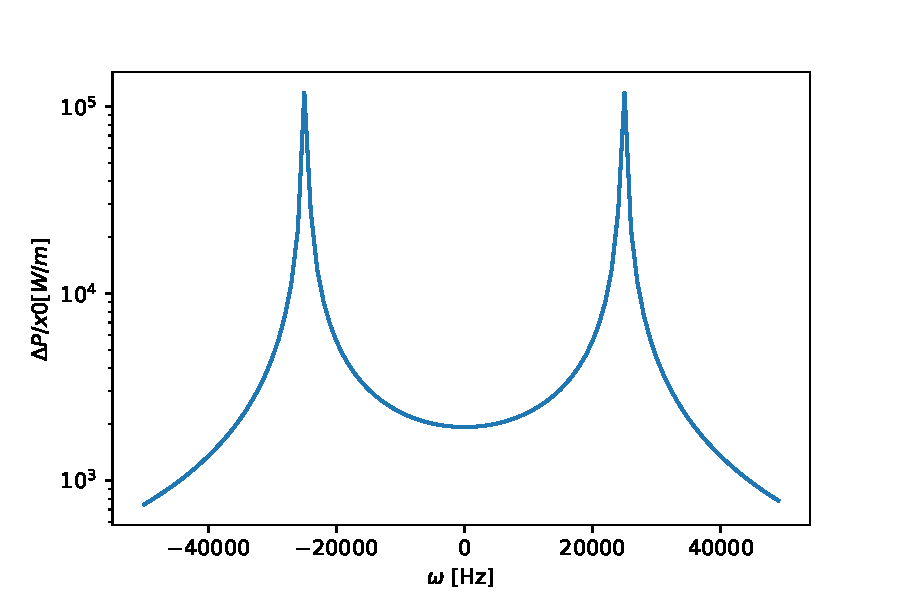
\includegraphics[width =1\columnwidth]{2b}
\caption{The transfer function $\Delta /x_0$ as a function of mirror modulation frequency $\omega$ for the Fabry-Perot Cavity.
}
\label{fig:2b}
\end{figure}

\item[\bf c)] {\bf Now write down a larger Adjacency Matrix which represents a Michelson interferometer with Fabry-Perot cavities in place of the usual end mirrors. Assume that there is a small asymmetry in the Michelson, such that the distance from the beamsplitter to one of the FP cavities is 100\,pm larger than the distance to the other cavity.
Make a Bode plot of the \emph{transfer function} as in part b), but instead of the transmission of the FP cavity, use the anti-symmetric (detection) port as the readout.}

\begin{figure}[t]
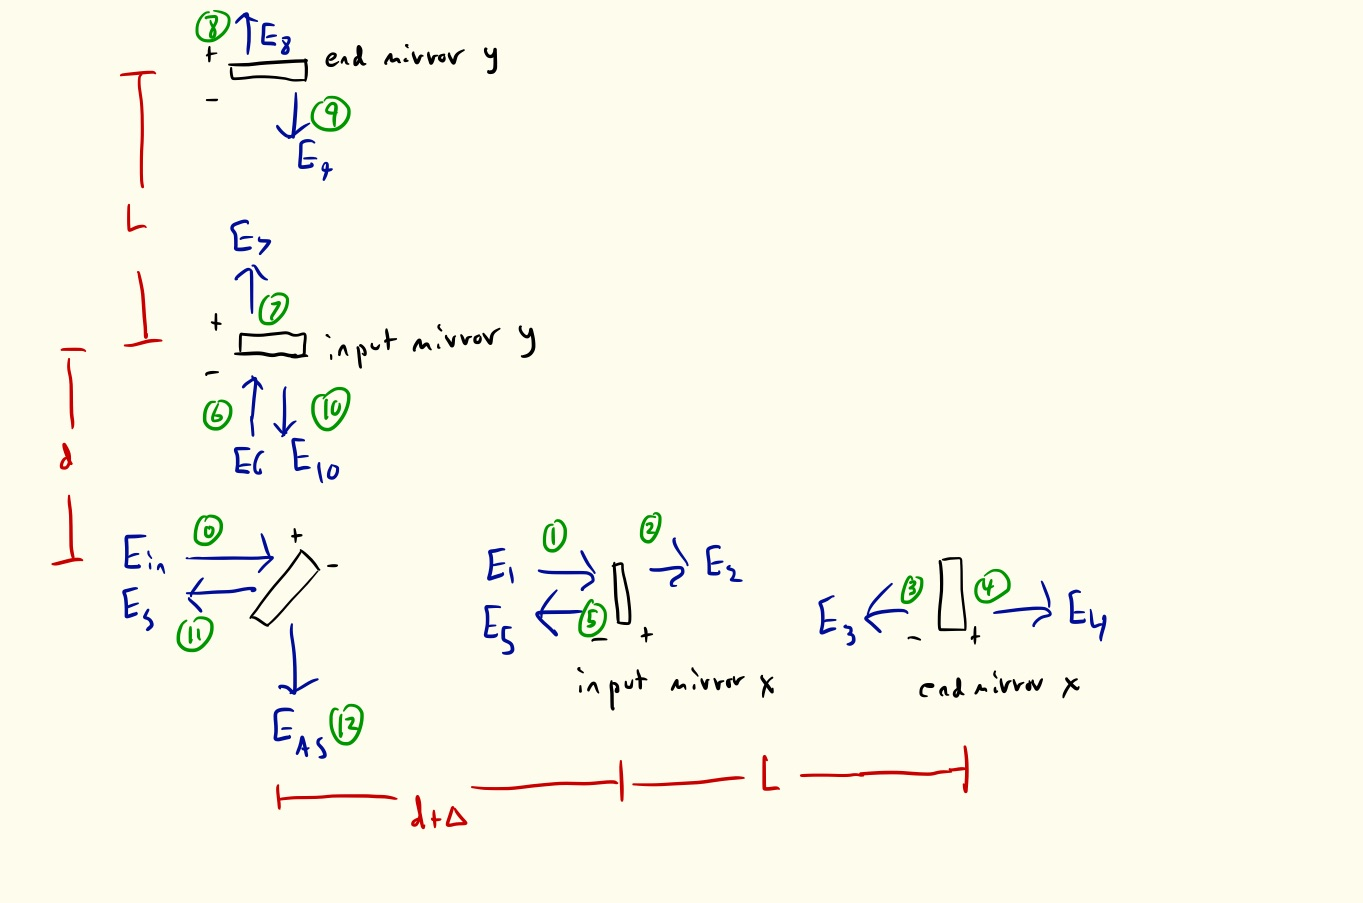
\includegraphics[width =1\columnwidth]{Michelson}
\caption{The transfer function $\Delta /x_0$ as a function of mirror modulation frequency $\omega$ for the Fabry-Perot Cavity.
}
\label{fig:Michelson}
\end{figure}

\begin{figure}[t]
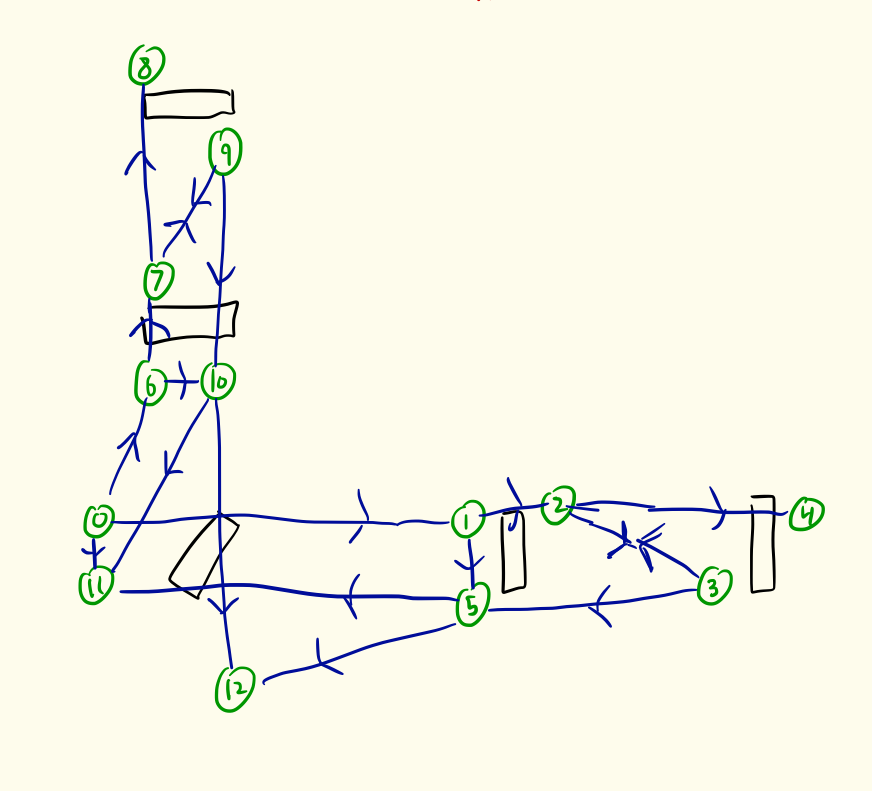
\includegraphics[width =1\columnwidth]{Michelsongraph}
\caption{The transfer function $\Delta /x_0$ as a function of mirror modulation frequency $\omega$ for the Fabry-Perot Cavity.
}
\label{fig:Michelsongraph}
\end{figure}

The optical layout of the Michelson interferometer is shown in figure \ref{fig:Michelson} and the corresponding directed graph is shown in figure \ref{fig:Michelsongraph}. We take the mirrors in each Fabry-Perot cavity to be identical. We assume the y-axis FP cavity is located a distance d from the beam splitter\footnote{The field at the antisymmetric port depends on d when $\Delta \neq 0$, but that the power does not. Hence we will set $d=0$ in our numerical computations of the power.} and the the x-cavity is located a distance $d+\Delta$ from the beam splitter with $\Delta =100\,pm$. We take the transmissivity and reflectivity of the beam splitter to be $t_{\rm BS}=r_{\rm BS}=1/\sqrt{2}$.


We now imagine that the x-axis end mirror is shaken about its central location with $\delta L= x_0\cos\omega t$. Using the results of problem 2 (a) and the logic of 2 (b), this means that the field at the anti-symmetric port is now the field at the carrier frequency plus the result of injecting the field (including the full time dependence)
\begin{align}
E_{side}(t)=ir_E\frac{x_0\omega_0}{c}(e^{i(\omega_0 +\omega)t}+e^{+i(\omega_0-\omega )t})G_{20}(\omega_0)E_{\rm in}
\end{align}
in node 3. Again using the system matrix to propagate the fields, the field at the antisymmetric port is
\begin{align}
E_{AS}(t)&=G_{12,0}(\omega_0)E_{\rm In}e^{i\omega_0 t} \nonumber \\
&+G_{12,3}(\omega_0+\omega)ir_EG_{20}(\omega_0)x_0\frac{\omega_0}{c}E_{\rm In}e^{i(\omega+\omega_0)t}
+G_{12,3}(\omega_0-\omega)ir_EG_{20}(\omega_0)x_0\frac{\omega_0}{c}E_{\rm In}e^{i(-\omega+\omega_0)t}, \label{eq:EASmod}
\end{align}
which is exactly of the same form of the field as the transmitted field from the modulated Fabry-Perot Cavity, with the exception that we have relabeled the elements of the system matrix to correspond to the correct nodes. Hence, the same logic as above reveals that the power at the antisymmetric port is
\begin{align}
P_T=|G_{12,0}(\omega_0)|^2P_{\rm In}+\Delta P\cos(\omega t+\phi),
\end{align}
where 
\begin{align}
\Delta P e^{i\phi}&=2G^*_{12,0}(\omega_0)ir_Ex_0\frac{\omega_0}{c}G_{12,3}(\omega_0+\omega)G_{20}(\omega_0)+2G_{12,0}(\omega_0)(ir_Ex_0\frac{\omega_0}{c}G_{12,3}(\omega_0-\omega)G_{20}(\omega_0))^*P_{\rm In} \nonumber \\
&=2ir_Ex_0\frac{\omega_0}{c}\left[G^*_{12,0}(\omega_0)G_{12,3}(\omega_0+\omega)G_{20}(\omega_0)-G_{12,0}(\omega_0)G^*_{12,3}(\omega_0-\omega)G^*_{20}(\omega_0)\right]P_{\rm in},
\end{align}


Labeling the nodes as in figure \ref{fig:Michelsongraph} the nonzero components of the adjacency matrix A are 
\begin{align}
&A_{10}=t_{BS}e^{-i\phi_x} & \nonumber \\
&A_{21}=t_I, & &A_{23}=r_Ie^{-i\phi}&  \nonumber \\
&A_{32}=-r_Ee^{-i\phi}& \nonumber  \\
&A_{42}=t_Ee^{-i\phi}& \nonumber \\
&A_{51}=-r_I, & &A_{53}=t_I \ep& \nonumber \\
&A_{60}=-r_{BS}e^{-i\phi_y}& \nonumber \\
&A_{76}=t_I,& &A_{7,9}=r_I\ep& \nonumber \\
&A_{87}=t_E\ep,& \nonumber \\
&A_{97}=-r_E\ep,& \nonumber \\
&A_{10,6}=-r_I,& 
&A_{10,9}=t_I\ep,& \nonumber \\
&A_{11,5}=t_{BS}e^{-i\phi_x},&
&A_{11,10}=-r_{BS}e^{-i\phi_y}& \nonumber \\
&A_{12,5}=r_{BS}e^{-i\phi_x},&
&A_{12,10}=t_{BS}e^{-i\phi_y}&,
\end{align}
where the phases are
\begin{align}
\phi(\omega)&=\omega L/c \nonumber \\ 
\phi_y(\omega)&=\omega d/c \nonumber  \\
\phi_x(\omega) &=\omega(d+\Delta)/c
\end{align}

Using the above adjacency matrix, the attached python code computes $\Delta P/x_0$. Figure \ref{fig:2c} shows  $\Delta P/x_0$ as a function of modulation frequency $\omega$ for the parameters given in the problem.
\begin{figure}[h]
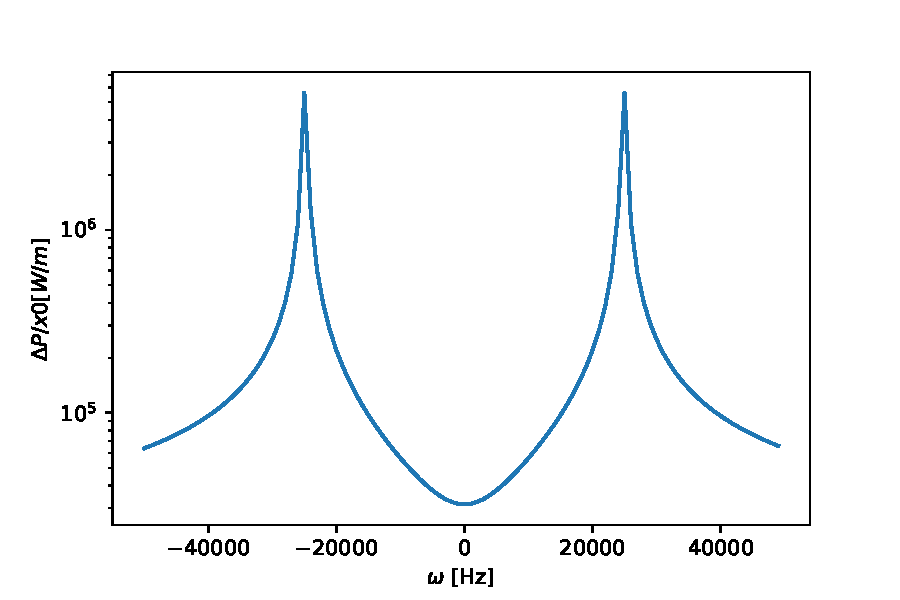
\includegraphics[width =1\columnwidth]{2c}
\caption{The transfer function $\Delta /x_0$ as a function of mirror modulation frequency $\omega$ for the Michelson Interferometer
}
\label{fig:2c}
\end{figure}


\end{itemize}

\end{enumerate}

\bigskip
{\color{Sepia} \hrule}
\end{document}
